\chapter{GraphCut-Flow}
\label{chapter:graphcut-flow}

In the previous chapter we've defined the concept of unbalanced coefficient that motivate us to introduce the PotentialFlow model. In fact, the unbalance coefficient is also present in the FlipFlow energy and it seems that its computation is the core of the shapes evolution presented so far. We confirm this hypothesis once more in this chapter. We present a graph model based on unbalance coefficients that converge to the digital shape of global optimum in the free digital Elastica problem. Moreover, the model can be easily modified for doing image segmentation.

\section{Graph-cut model}

Let $S$ a digital shape. Similarly to previous chapters, we denote $S^{(k)}$ the $k$-th shape produced by the model. If $k$ is ommited, we assume $k=0$. Given $m>0$, The optimization set $O$ is defined as

\begin{align*}
	O^{(k)} &:=\left\{ p \in \Omega \; | \; -m <= d_{S^{(k)}}(p) \leq m \right\}\\
\end{align*}

We are going to construct a graph $G(V,E)$ from $S$. Its vertex set is defined as

\begin{align*}
	V&= \{ v_p \; | \; p \in S \} \cup \{s,t\}.
\end{align*}

The vertices $s,t$ are denoted the source and target vertices, respectively, and do not correspond to any point in $S$. We define an edge as a pair of vertices and a weight value, i.e., the triple $(v_1,v_2,w)$ denotes an edge from vertex $v_1$ to $v_2$ with weight $w$. The edge set of $G$ is defined as

\begin{align*}
	E_1 &= \{ (v_p,v_q,w(p,q)) \; | \; \forall p \in O(S) \quad q \in \mathcal{N}_{4}(p) \}\\
	E_2 &= \{ (s,v_p,M) \; | \; \forall p \in S \setminus O(S) \} \\
	E_3 &= \{ (v_p,t,M) \; | \; \forall p \in \overline{S} \setminus O(S) \} \\
	E &= E_1 \cup E_2 \cup E_3,
\end{align*}

where $w(p,q) = u(S,p) + u(S,q)$ and $M=\pi^2 R^4$. 

\begin{definition}{Cut set}
 A cut set of a graph $G(V,E)$ is a subset $E' \subset E$ such that source and target vertices are not connected in $G(V,E \setminus E')$. The value of a cut is defined as
 
 \begin{align*}
 	v(E') &= \sum_{e \in E'}{w(e)}.
 \end{align*}
 
\end{definition}

Cuts are a natural way to partition a digital shape in two disjoint sets. In the GrabCut algorithm, the images are partitioned in foreground and background. In the context of shape evolution, we partition the vertices in: belong to $S$ (connected to source) and do not belong to $S$ (connected to target).

The graph $G$ is built such that its minimum cut comprise the pixels with minimum sum of its unbalance coefficients. We denote $C_s^{(k)}$ ($C_t^{(k)}$) the source (target) component of the graph induced by the minimum cut of $G$. 

\begin{definition}{$m$-graph-cut flow}

Given a natural number $m>0$ and digital set $S$, the $m$-graph-cut flow is defined as

\begin{align*}
	\left \{ S^{(k)} \; | \; \begin{array}{ll}
	S^{(0)}&=S \\
	S^{(k)}&= \{ p \; | \; v_p \in C_s^{(k)} \}
	\end{array} \right\}
\end{align*}

\end{definition}

The $m$-graph-cut flow produces similar results to the previous flows (see figure \ref{}), but is much faster to compute and implement. 

\begin{figure}
\begin{tabular}{cccc}
&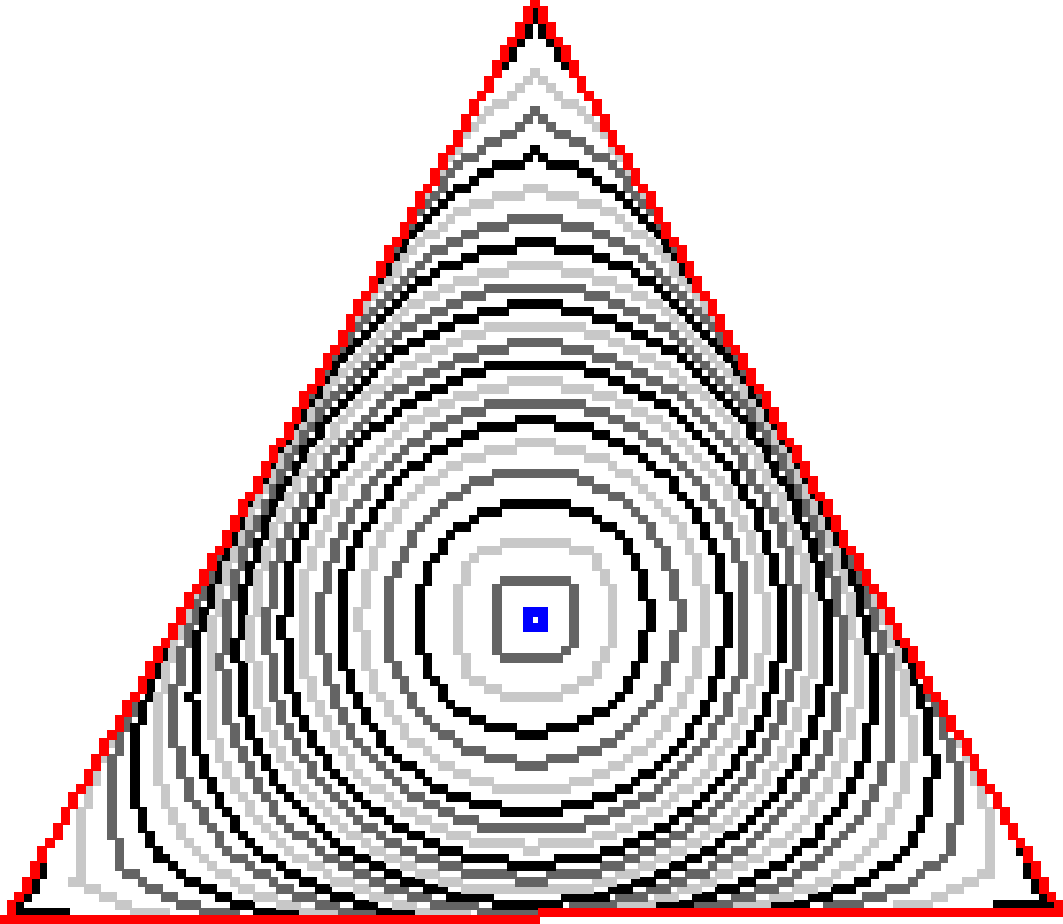
\includegraphics[scale=0.25]{figures/chapter8/graph-flow/triangle/neigh-0/summary.pdf} & 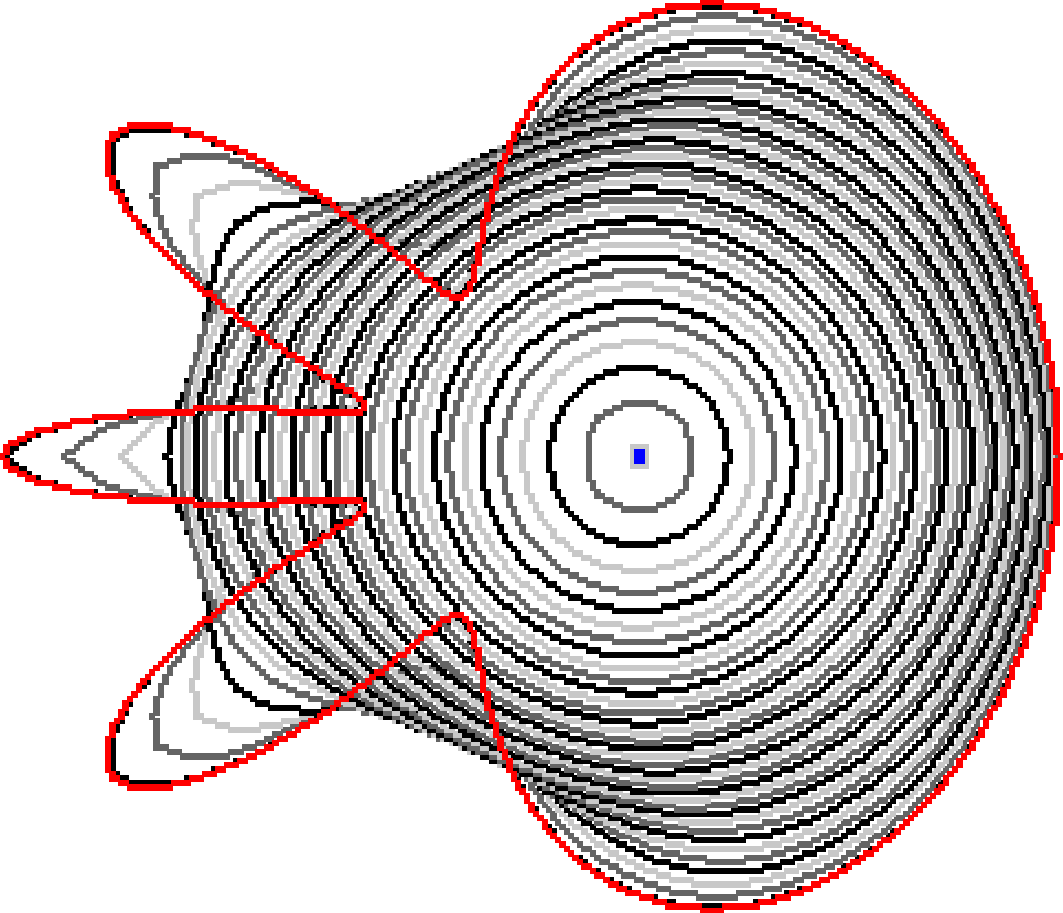
\includegraphics[scale=0.25]{figures/chapter8/graph-flow/flower/neigh-0/summary.pdf} & 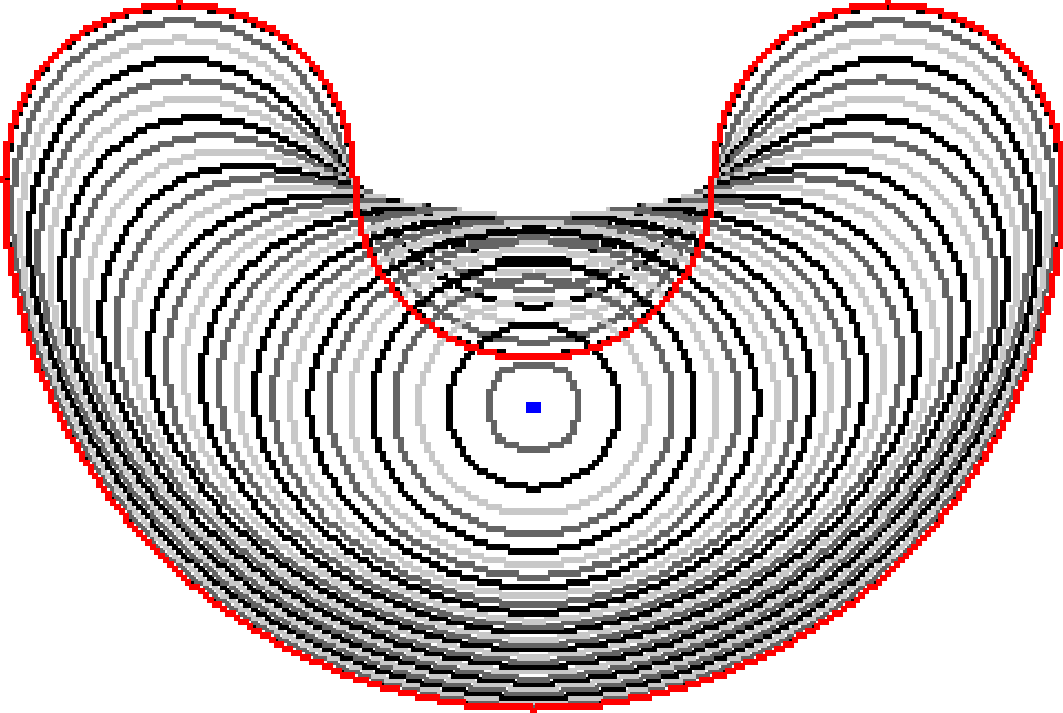
\includegraphics[scale=0.25]{figures/chapter8/graph-flow/bean/neigh-0/summary.pdf}
\end{tabular}
\caption{$1$-GraphFlow results for the triangle, flower and bean shapes. Differently from the previous models, the GraphFlow evolves the shape to a single point for any value of $m$. However, for higher values of $m$ the convergence is faster. Shapes are displayed at every $10$ iterations.}
\label{fig:graph-flow-neigh0-results}
\end{figure}

\section{LSGC algorithm}
	We present a local-search strategy for the GraphFlow model. The idea is to define a neighborhood for shape $S^{(k)}$ and compute the GraphFlow model for each of its members. The next shape $S^{(k+1)}$ is chosen as the one with lower digital Elastica.

\begin{definition}{$a$-neighborhood explorer set}
	Let $S$ a digital set and $a$ a natural number. Its $a$-neighborhood explorer set is defined as
	\begin{align*}
		N_a(S) &= S \cup \bigcup_{a' < a}{S^{+a} \cup S^{-a}},
	\end{align*}
	where $S^{+a}$($S^{-a}$) denotes a dilation(erosion) by a square of side $a$.
\end{definition}

The local-enumerative graph-cut (LEGC) algorithm is described as


\begin{algorithm}
 \SetKwData{It}{k}
 \SetKwData{MIt}{maxIt}
 \SetKwData{Delta}{delta}
 \SetKwInOut{Input}{input}\SetKwInOut{Output}{output}
 \SetKwComment{comment}{//}{}
 
 \Input{A digital set $S$; the optimization band $m$; the neighborhood explorer set size $a$ ; the maximum number of iterations \MIt;}
 \BlankLine
 $S^{(0)} \longleftarrow S$\;
 $k \longleftarrow 1$\;
 \While{ \It $<$ \MIt  }{ 	
	$candidates \longleftarrow \{\}$\;
 	\ForEach{ $X \in N_a(S^{(k)})$ }
 	{
 		$candidates \longleftarrow candidates \cup \{ p \; | \; v_p \in C_s( X ) \}$\;
 	}
 
	$S^{(k)} \longleftarrow \displaystyle \argmin_{X \in candidates}{ \hat{E}(X) }$\; 	
	\It $\longleftarrow$ \It $+1$\;
	
 }
 \caption{LSGC algorithm.}
 \label{alg:legc-algorithm}  
\end{algorithm}

The LSGC algorithm can grow or shrink accordingly with the $\alpha$ coefficient in the digital Elastica (see figure \ref{fig:graph-flow-neigh2-results}). For $a=0$, we recover the convergence to a point behaviour observed the in FlipFlow and PotentialFlow model. Moreover, its solution for the free Elastica problem is very similar to those given by the enumerative process of chapter \ref{chapter:digital-elastica}, i.e., the shapes converges to the expected global optimum. However, for the constrained Elastica problem, the LSGC encounters some difficulties to evolve (see figure \ref{fig:graph-flow-constrained}). We believe that a larger neighborhood, possibly random, could solve the issue.

\begin{figure}
\begin{tabular}{cccc}
&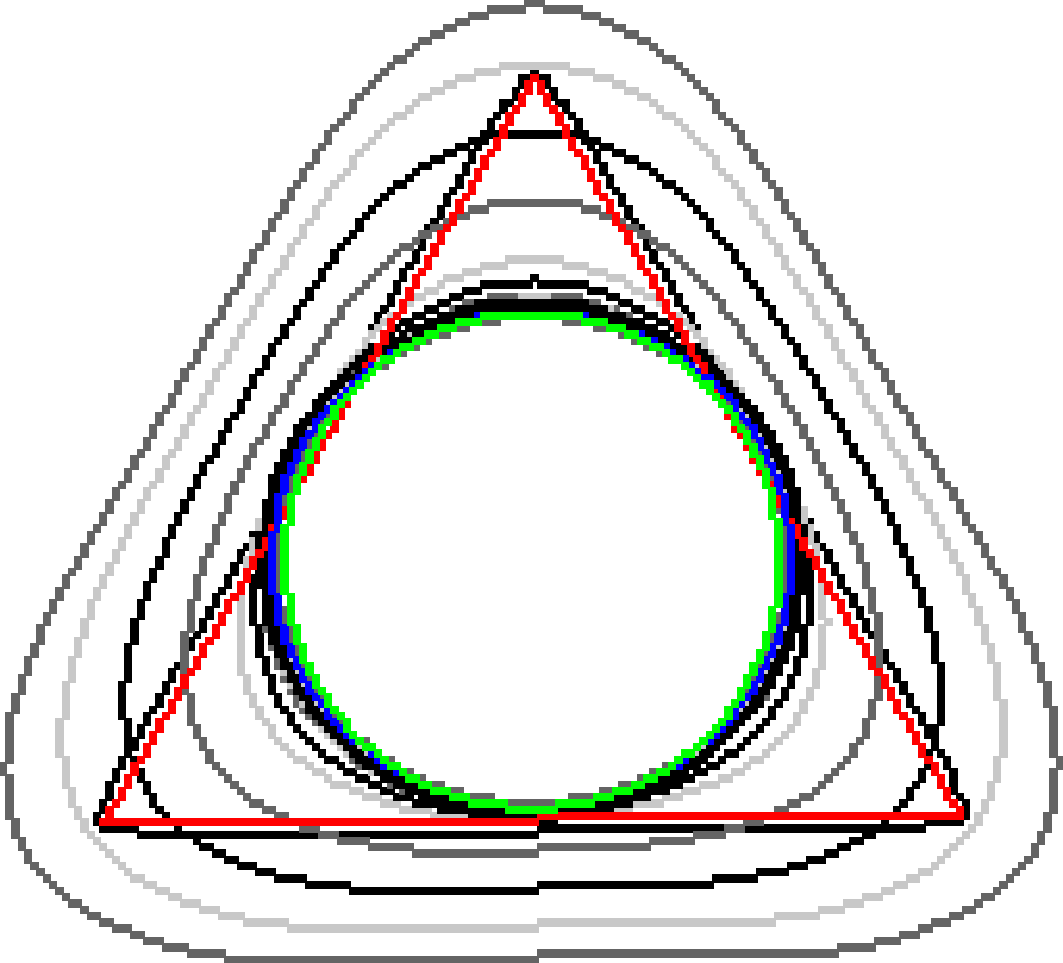
\includegraphics[scale=0.25]{figures/chapter8/graph-flow/triangle/neigh-2/summary.pdf} & 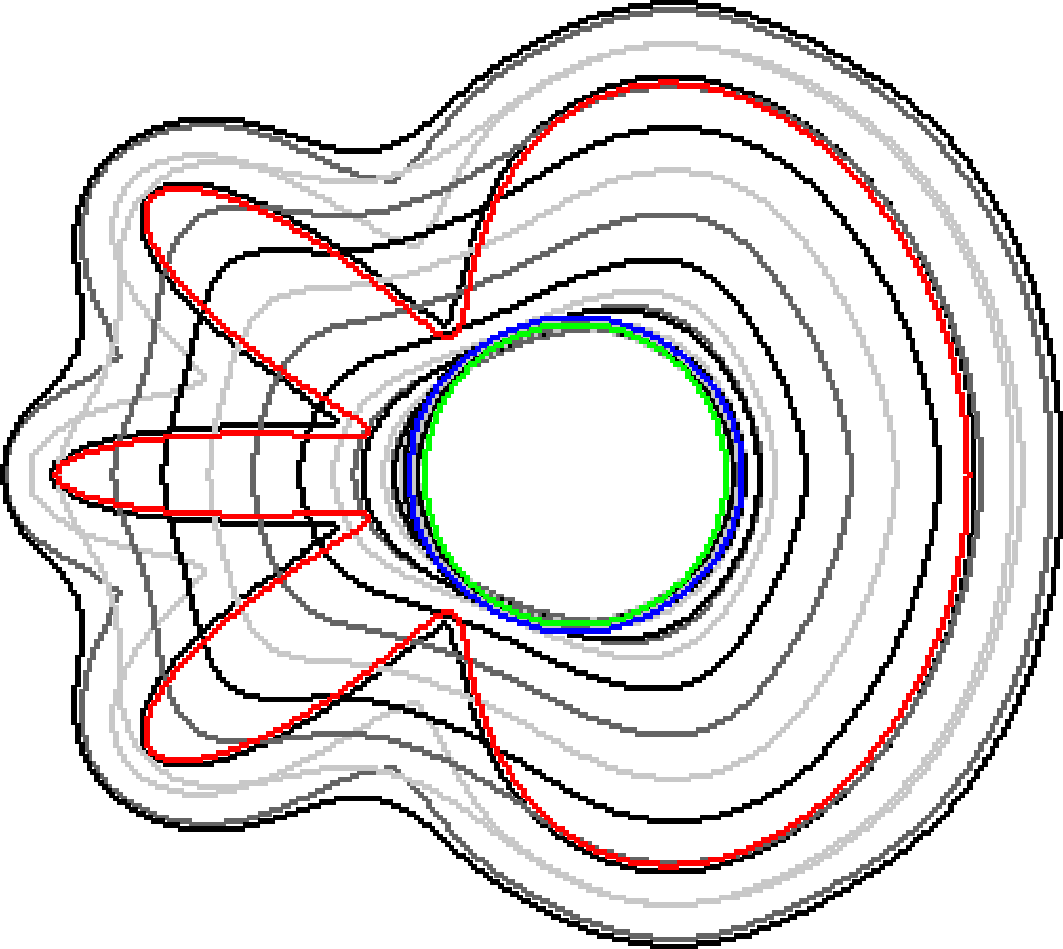
\includegraphics[scale=0.25]{figures/chapter8/graph-flow/flower/neigh-2/summary.pdf} & 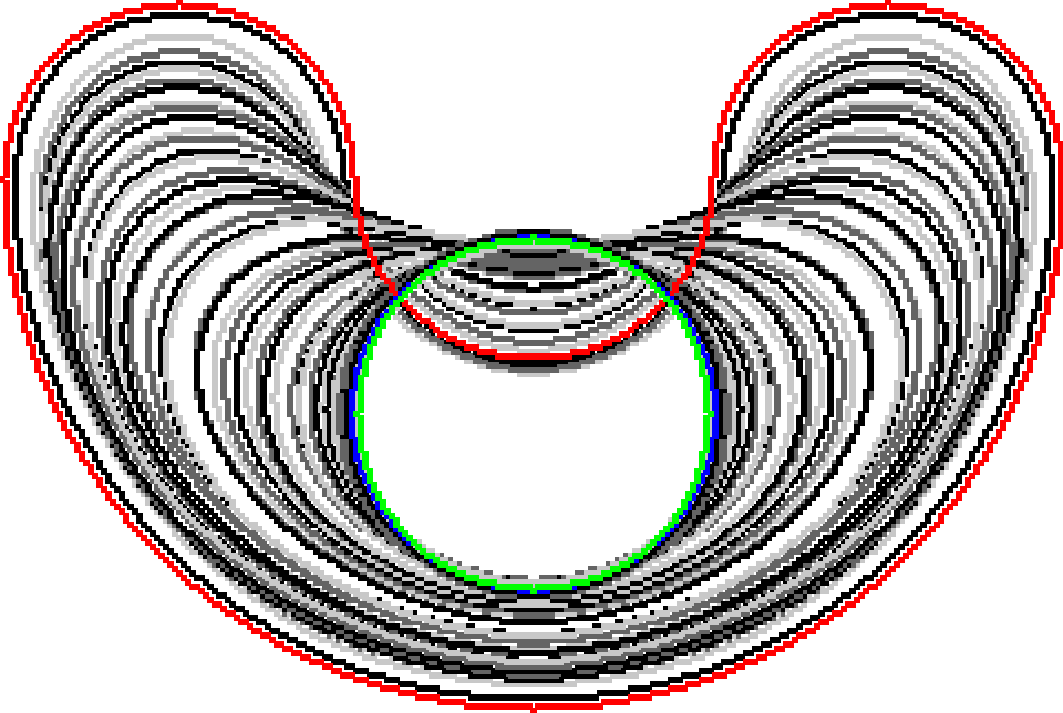
\includegraphics[scale=0.25]{figures/chapter8/graph-flow/bean/neigh-2/summary.pdf}
\end{tabular}
\caption{The LSGC algorithm can shrink and grow, and it converges to the global optimum (green curve) in the free Elastica problem. For the flows in the figure, we are using $a=2$ and shapes are displayed at every $10$ iterations.}
\label{fig:graph-flow-neigh2-results}
\end{figure}


\begin{figure}
\begin{tabular}{ccc}
&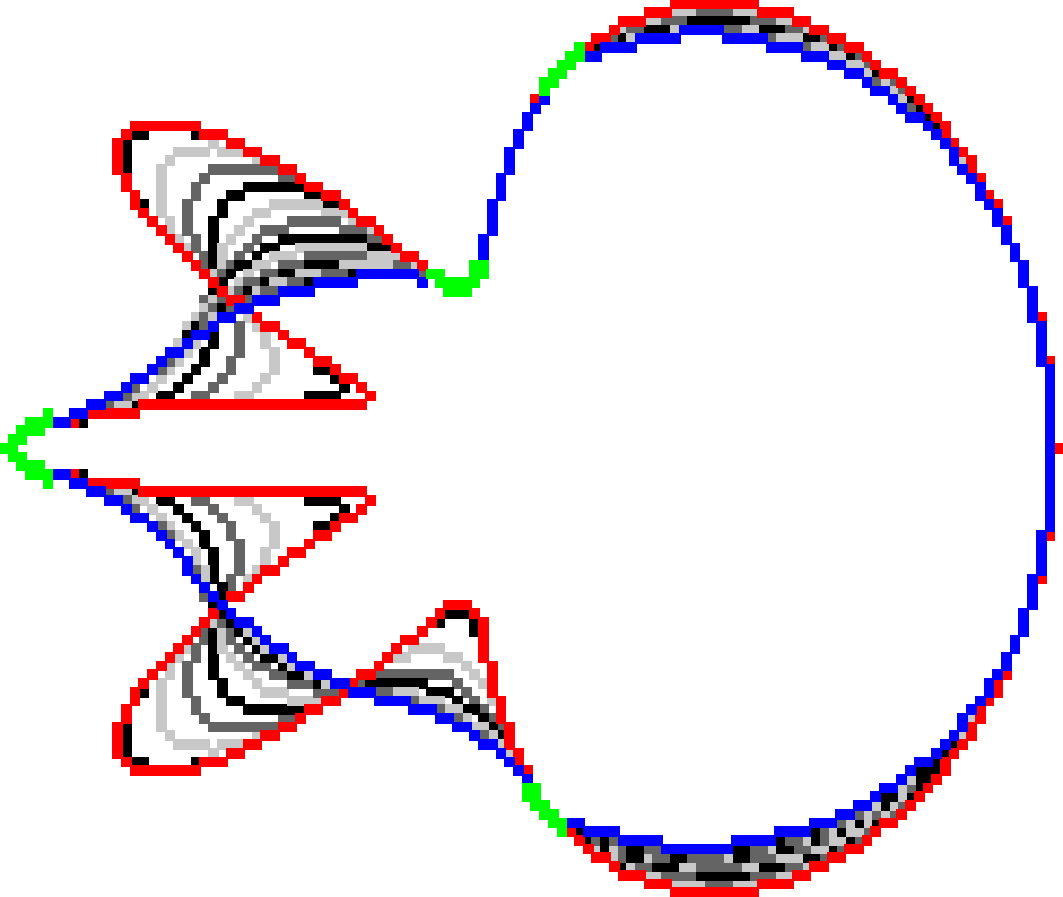
\includegraphics[scale=0.4]{figures/chapter8/constrained-elastica/flower-1/lp-0.001/summary.pdf} & 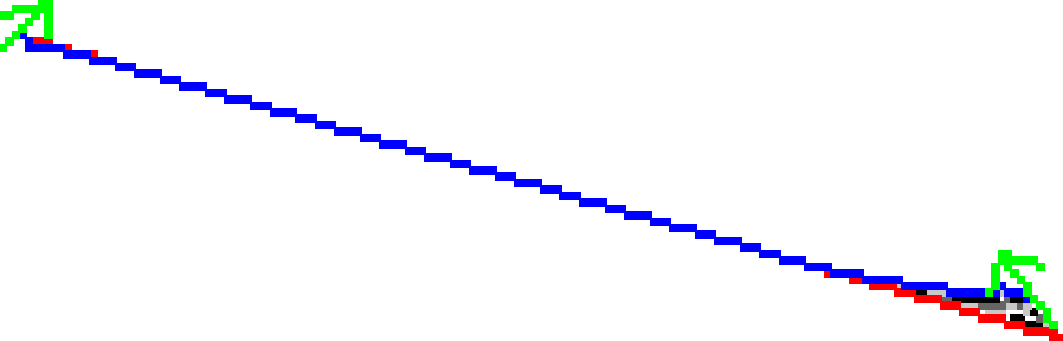
\includegraphics[scale=0.4]{figures/chapter8/constrained-elastica/curve-3/lp-0.001/summary.pdf}
\end{tabular}
\caption{The LSGC encounters some difficulties to evolve the shapes in the constrained Elastica problem. We think that a larger, possibly random, neighborhood may solve the problem. For both flows in the figure, we are using $a=2$.}
\label{fig:graph-flow-constrained}
\end{figure}

\section{Injecting data term}

The state-of-art image segmentation by graph-cut is given by the GrabCut algorithm. The GrabCut model incorporates two data term components, one related to the boundary, and the other to the region. Several works tried to inject geometric information in a graph-cut framework for image segmentation. While some works sucessfuly injected perimeter information, those that attempt to include curvature suffer from lack of precision or running time complexity. In this section we propose a model that advances in these two criterias.
